\documentclass[11pt,a4paper]{article}

\usepackage[T1]{fontenc}
\usepackage[utf8]{inputenc}
\usepackage{lmodern}
\usepackage[margin=24mm]{geometry}
\usepackage{microtype}
\usepackage{amsmath,amssymb}
\usepackage{graphicx}
\usepackage{booktabs}
\usepackage{longtable}
\usepackage{tabularx}
\usepackage{array}
\usepackage{float}
\usepackage{caption}
\usepackage{xcolor}
\usepackage[hidelinks]{hyperref}

\graphicspath{{figures/}}
\setlength{\parindent}{0pt}
\setlength{\parskip}{0.55em}
\captionsetup{font=small,labelfont=bf,justification=raggedright,singlelinecheck=false}
\renewcommand{\arraystretch}{1.05}
\newcommand{\method}{PMRC}
\newcommand{\vect}[1]{\mathbf{#1}}
\newcommand{\indicator}{\mathbf{1}}

\title{Supplementary Material for\\
Post-hoc Prototype-Margin Reliability Calibration for Closed-Set Selective Fine-Grained Recognition under Label Noise}
\author{Xianning Zhao, Haoyuan Tang, and Liang Qiao\\
School of Information Science and Engineering\\
Lanzhou University, Lanzhou 730000, Gansu, China\\
\texttt{zhxianning2025@lzu.edu.cn}}
\hypersetup{
  pdftitle={Supplementary Material for Post-hoc Prototype-Margin Reliability Calibration for Closed-Set Selective Fine-Grained Recognition under Label Noise},
  pdfauthor={Xianning Zhao, Haoyuan Tang, Liang Qiao}
}
\date{}

\begin{document}
\maketitle

\section{Calibration stability}

\begin{figure}[H]
  \centering
  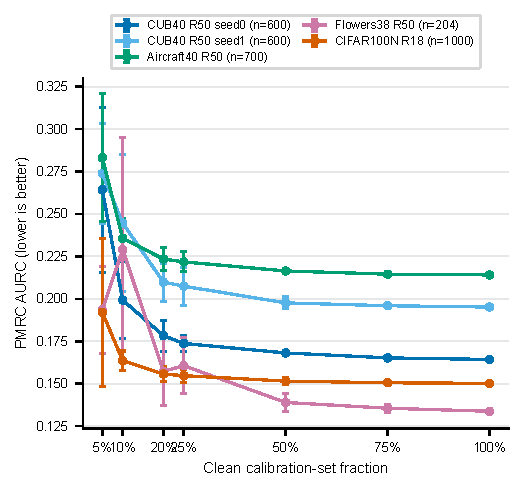
\includegraphics[width=0.88\textwidth]{figureS1_stability.pdf}
\caption{Calibration-set-size stability. Each curve reports \method{} AURC after random subsampling of the clean calibration set to 5\%, 10\%, 20\%, 25\%, 50\%, 75\%, or 100\% of its original size. Symbols show means over ten repeated subsets where applicable, and error bars show one standard deviation. The complete calibration point has no sampling variance. Performance and variance degrade sharply below 20\%.}
  \label{fig:s1}
\end{figure}

\section{Evaluation protocols}

\begin{table}[H]
\centering
\caption{Evaluation protocols. The controlled matrix contains CUB-200-2011,
FGVC-Aircraft, Oxford Flowers102, and CIFAR-100N. WebFG uses the official web
training labels and one fixed clean calibration/test partition per subset.}
\label{tab:evaluation-protocols}
\small
\begin{tabularx}{\textwidth}{@{}lXrr@{}}
\toprule
Evaluation & Noise or supervision & Calibration & Test \\
\midrule
CUB semantic-20 / 40 & top-5 semantic-neighbor replacement & 600 & 5,794 \\
CUB symmetric-40 & uniform closed-set replacement & 600 & 5,794 \\
Aircraft semantic-20 / 40 & top-5 semantic-neighbor replacement & 700 & 3,333 \\
Flowers semantic-25 / 37.5 & top-5 semantic-neighbor replacement & 204 & 6,149 \\
CIFAR-100N & real human annotation noise (40.2\%) & 1,000 & 10,000 \\
Stanford Dogs & top-5 semantic-neighbor replacement (40\%) & 600 & 6,174 \\
WebFG bird & official web labels; six seeds & 584 & 5,210 \\
WebFG aircraft & official web labels; three seeds & 300 & 3,033 \\
WebFG car & official web labels; three seeds & 783 & 7,258 \\
\bottomrule
\end{tabularx}
\end{table}

\section{Training-objective transfer}

CE seeds 1--2 and GCE seeds 0--2 were trained after the primary matrix was
complete. All completed seeds are reported; no seed was removed after observing
its test result.

\begin{table}[H]
\centering
\caption{Matched CUB semantic-40 ResNet-50 runs across training objectives. Architecture, data splits, prototype construction, and the post-hoc protocol are held fixed. The nine-run comparison reuses CE seed 0 and ELR seeds 0--2 from the primary matrix and adds CE seeds 1--2 and GCE seeds 0--2. Improvement is the per-seed relative AURC reduction, averaged within each objective.}
\label{tab:training-objective-transfer}
\small
\begin{tabular}{@{}lrrrrr@{}}
\toprule
Objective & Seeds & MSP AURC & PMRC AURC & Improvement & Favorable \\ 
\midrule
Cross-entropy & 3 & 0.2327 & 0.1914 & +17.97 $\pm$ 4.60\% & 3/3 \\
ELR & 3 & 0.2109 & 0.1769 & +16.22 $\pm$ 4.63\% & 3/3 \\
GCE ($q=0.7$) & 3 & 0.2090 & 0.1725 & +17.47 $\pm$ 1.50\% & 3/3 \\
\bottomrule
\end{tabular}
\end{table}

All nine paired bootstrap intervals across the three objectives were below
zero. PMRC had lower AURC than Temperature, pNorm, KNN, and Trust Score in all
nine runs. The GCE seed-wise relative reductions were 19.11\%, 16.17\%, and
17.14\%.
The paired bootstrap interval for PMRC minus MSP excluded zero in every
GCE seed, and the mean within-MSP prototype AUROC was 0.727. PMRC also had
lower AURC than temperature scaling, pNorm, KNN, and Trust Score in all three
GCE runs. These runs extend the post-hoc transfer result beyond the original
ELR pipeline; they are not experiments with DGCL or CYFLOD.

\section{Independent downstream dataset and split transfer}

The protocol, class split, noise rule, and gate threshold were frozen before
training. The official test membership was unchanged. SHA-256 auditing found
120 duplicate train-side images that repeated a test image or another train
image; these were removed before splitting. The final manifest contains 13,686
training images, 600 clean validation/calibration images, and 6,174 test images
over all 120 classes.

\begin{table}[H]
\centering
\caption{Stanford Dogs downstream dataset and split transfer under 40\% semantic-neighbor
noise. Gate AUROC is computed on the clean validation split. PMRC is selected
when this value exceeds the frozen threshold 0.5.}
\label{tab:stanford-dogs-external}
\small
\begin{tabular}{@{}rrrrrrr@{}}
\toprule
Seed & Gate AUROC & MSP AURC & PMRC AURC & Relative gain & 95\% CI & Gate \\
\midrule
0 & 0.8526 & 0.0861 & 0.0614 & +28.63\% & [-0.0287,-0.0208] & PMRC \\
1 & 0.7854 & 0.0799 & 0.0588 & +26.46\% & [-0.0244,-0.0178] & PMRC \\
2 & 0.8162 & 0.0897 & 0.0627 & +30.11\% & [-0.0317,-0.0230] & PMRC \\
Mean & 0.8181 & 0.0852 & 0.0610 & +28.40\% & -- & 3/3 \\
\bottomrule
\end{tabular}
\end{table}

All three paired intervals exclude zero, and the gate direction matches the
direct PMRC effect in all three runs. PMRC also has lower AURC than all four
selective baselines in every seed. Their mean values are 0.0801 for
Temperature, 0.0809 for pNorm, 0.0743 for KNN agreement, and 0.1237 for Trust
Score, compared with 0.0610 for PMRC. Selective risk at 90\% coverage decreases
in every seed, with a mean reduction from 0.1858 to 0.1650. This experiment
uses an independent downstream fine-grained dataset under synthetic semantic
noise. Stanford Dogs is derived from ImageNet, so this experiment isolates
downstream dataset and split transfer. It does not isolate ImageNet pretraining
exposure; a pretraining-independent real-web label domain remains outside this
test.

\section{WebFG seed-level results}

Seeds 0--2 are the initial WebFG runs. The initial Bird seeds were heterogeneous
and all selected MSP. Before inspecting the PMRC results for seeds 3--5, we
registered three additional Bird seeds to test whether this fallback regime was
reproducible. The protocol fixed the split, classifier configuration, epoch
count, gate threshold, and evaluation metrics, and required all three added
seeds to be reported without replacement. All seeds share the same clean
calibration/test partition within a subset.

\begin{table}[H]
\centering
\caption{WebFG seed-level selective results. CI is a paired bootstrap interval for the PMRC-minus-MSP AURC difference over test images; negative values favor PMRC.}
\label{tab:webfg-seed-level}
\footnotesize
\setlength{\tabcolsep}{4pt}
\begin{tabular}{@{}lllrrrr@{}}
\toprule
Subset & Seed & Set & MSP & PMRC & Rel. change & 95\% CI \\
\midrule
Bird & 0 & initial & 0.07336 & 0.07424 & -1.20\% & [-0.0012,+0.0029] \\
Bird & 1 & initial & 0.07839 & 0.07891 & -0.67\% & [-0.0020,+0.0028] \\
Bird & 2 & initial & 0.08388 & 0.08219 & +2.01\% & [-0.0056,+0.0018] \\
Bird & 3 & replication & 0.07615 & 0.07840 & -2.96\% & [+0.0004,+0.0043] \\
Bird & 4 & replication & 0.07438 & 0.07441 & -0.04\% & [-0.0022,+0.0021] \\
Bird & 5 & replication & 0.07767 & 0.07781 & -0.19\% & [-0.0015,+0.0019] \\
Aircraft & 0 & initial & 0.11561 & 0.11312 & +2.15\% & [-0.0049,-0.0002] \\
Aircraft & 1 & initial & 0.13252 & 0.13031 & +1.67\% & [-0.0048,+0.0005] \\
Aircraft & 2 & initial & 0.11270 & 0.10742 & +4.68\% & [-0.0086,-0.0022] \\
Car & 0 & initial & 0.08533 & 0.08123 & +4.81\% & [-0.0058,-0.0021] \\
Car & 1 & initial & 0.07616 & 0.07496 & +1.57\% & [-0.0033,+0.0010] \\
Car & 2 & initial & 0.07683 & 0.07426 & +3.35\% & [-0.0048,-0.0007] \\
\bottomrule
\end{tabular}
\end{table}

\section{Prototype-source controls}

\begin{table}[H]
\centering
\caption{Prototype-source control results. The clean-label oracle is diagnostic only and is not a deployable method.}
\label{tab:prototype-source}
\footnotesize
\setlength{\tabcolsep}{3pt}
\begin{tabularx}{\textwidth}{@{}Xrrrrr@{}}
\toprule
Setting & No prototype & Noisy prototype & Clean oracle & ImageNet prototype & Shuffled \\
\midrule
CUB semantic-40 (3 seeds) & 0.2052 & 0.1769 & 0.1466 & 0.1812 & 0.2046 \\
Aircraft semantic-40 & 0.2337 & 0.2153 & 0.1830 & 0.2300 & 0.2341 \\
Flowers102 semantic-37.5 & 0.1674 & 0.1347 & 0.0966 & 0.1292 & 0.1625 \\
\bottomrule
\end{tabularx}
\end{table}

Noisy-label prototypes beat the no-prototype and shuffled controls in all five runs. They beat ImageNet-feature prototypes in three of five runs. Clean-label prototypes were better in every run but require labels unavailable in the practical setting.

\section{Risk-constrained coverage}

\begin{table}[H]
\centering
\caption{Empirical risk-constrained coverage across 42 evaluations. Calibration thresholds are selected from clean validation data and applied to fixed test sets. The final two columns count test runs whose realized risk exceeds the target. These results are not a distribution-free guarantee.}
\label{tab:risk-supp}
\footnotesize
\setlength{\tabcolsep}{3pt}
\begin{tabular}{@{}rrrrr@{}}
\toprule
Target & Higher PMRC coverage & Mean gain & MSP risk$>$target & PMRC risk$>$target \\
\midrule
5\% & 36/42 & +7.7 pp & 24/42 & 26/42 \\
10\% & 38/42 & +8.3 pp & 21/42 & 25/42 \\
15\% & 37/42 & +7.5 pp & 19/42 & 27/42 \\
\bottomrule
\end{tabular}
\end{table}

Exploratory paired McNemar exact tests over the fixed run set compare which run
exceeds each risk target under MSP versus PMRC. PMRC-only versus MSP-only
violations are 9 versus 7 ($p=0.804$) at 5\%, 9 versus 5 ($p=0.424$) at 10\%,
and 10 versus 2 ($p=0.039$) at 15\%. The 42 runs reuse datasets, seeds, and
training configurations, so these tests are descriptive rather than
population-level inference.

\section{Baseline calibration protocol}

\begin{table}[H]
\centering
\caption{Post-hoc baseline protocol. Every method uses the same clean calibration split and fixed test split, and no method uses test labels for fitting or hyperparameter selection.}
\label{tab:baseline-protocol}
\small
\begin{tabularx}{\textwidth}{@{}lXl@{}}
\toprule
Method & Calibration operation & Test labels used \\
\midrule
Temperature scaling & Temperature fitted by calibration NLL & No \\
MaxLogit-pNorm & Power $p\in\{1,\ldots,10\}$ selected by calibration AURC & No \\
KNN agreement & Neighbor count $k\in\{1,5,10,20\}$ selected by calibration AURC & No \\
Trust Score & Neighbor count $k\in\{1,5,10,20\}$ selected by calibration AURC & No \\
\method{} & Ten-descriptor logistic calibrator; L2 strength selected by five-fold calibration CV & No \\
\bottomrule
\end{tabularx}
\end{table}

\section{Calibration robustness}

All perturbation experiments reuse the frozen classifiers. The L2 regularization selected for each clean run is fixed across perturbations, so the reported changes isolate calibration-label or class-coverage degradation.

\begin{table}[H]
\centering
\caption{Calibration-label noise and missing-class stress tests. Each non-clean condition contains five repetitions over 40 classifiers.}
\label{tab:calibration-robustness}
\small
\setlength{\tabcolsep}{4pt}
\begin{tabular}{@{}lrrrr@{}}
\toprule
Condition & Evaluations & Direct gain & Gated gain & Gated non-regression \\
\midrule
Clean calibration & 40 & +9.6\% & +9.7\% & 100.0\% \\
5\% label corruption & 200 & +9.1\% & +9.2\% & 99.0\% \\
10\% label corruption & 200 & +8.1\% & +8.3\% & 97.5\% \\
20\% label corruption & 200 & +6.3\% & +6.7\% & 88.0\% \\
10\% missing classes & 200 & +9.4\% & +9.5\% & 99.5\% \\
25\% missing classes & 200 & +9.0\% & +9.1\% & 97.0\% \\
50\% missing classes & 200 & +7.4\% & +7.6\% & 89.0\% \\
\bottomrule
\end{tabular}
\end{table}

\section{Class-disjoint calibration}

For each repeat, 20\% or 40\% of classes were excluded from calibration and used only for evaluation. All classifier parameters were frozen.

\begin{table}[H]
\centering
\caption{Gate and calibration transfer on unseen classes. Gains are relative AURC reductions. Gated non-regression counts outcomes no worse than MSP.}
\label{tab:class-disjoint}
\small
\setlength{\tabcolsep}{4pt}
\begin{tabular}{@{}lrrrrr@{}}
\toprule
Dataset & Held-out classes & Evaluations & Direct gain & Gated gain & Gated non-regression \\
\midrule
Aircraft & 20\% & 30 & +11.4\% & +11.4\% & 100.0\% \\
Aircraft & 40\% & 30 & +12.3\% & +12.3\% & 100.0\% \\
CIFAR-100N & 20\% & 15 & +4.9\% & +4.9\% & 93.3\% \\
CIFAR-100N & 40\% & 15 & +4.0\% & +4.0\% & 100.0\% \\
CUB & 20\% & 65 & +12.8\% & +12.8\% & 95.4\% \\
CUB & 40\% & 65 & +12.3\% & +12.3\% & 95.4\% \\
Flowers102 & 20\% & 30 & +12.4\% & +12.4\% & 83.3\% \\
Flowers102 & 40\% & 30 & +13.2\% & +13.2\% & 96.7\% \\
WebFG aircraft & 20\% & 15 & +1.6\% & +1.6\% & 60.0\% \\
WebFG aircraft & 40\% & 15 & +1.8\% & +1.5\% & 60.0\% \\
WebFG bird & 20\% & 30 & -1.8\% & +0.6\% & 100.0\% \\
WebFG bird & 40\% & 30 & -3.0\% & +0.2\% & 83.3\% \\
WebFG car & 20\% & 15 & +2.1\% & +2.1\% & 73.3\% \\
WebFG car & 40\% & 15 & +1.8\% & +1.8\% & 80.0\% \\
\bottomrule
\end{tabular}
\end{table}

\section{Finite-sample risk-control baseline}

\begin{table}[H]
\centering
\caption{Split Learn-then-Test comparison. Thresholds use Clopper--Pearson upper bounds with a 10\% family-wise confidence budget. Risk averages runs that accept at least one sample.}
\label{tab:ltt}
\small
\begin{tabular}{@{}lrrrr@{}}
\toprule
Target risk & Accepted MSP / PMRC & MSP coverage & PMRC coverage & PMRC test risk \\
\midrule
5\% & 0/42 / 1/42 & 0.0\% & 0.6\% & 1.8\% \\
10\% & 15/42 / 22/42 & 15.4\% & 22.2\% & 4.3\% \\
15\% & 27/42 / 37/42 & 31.8\% & 43.4\% & 7.8\% \\
\bottomrule
\end{tabular}
\end{table}

Among runs that accepted at least one sample, no MSP or PMRC threshold
exceeded its target risk at the 5\%, 10\%, or 15\% budget.

\section{Decision cost}

\begin{table}[H]
\centering
\caption{Expected decision cost when one classification error has unit cost. Thresholds are selected on calibration data and evaluated on test data.}
\label{tab:decision-cost}
\small
\begin{tabular}{@{}rrrrrr@{}}
\toprule
Rejection cost & MSP cost & PMRC cost & PMRC lower & MSP coverage & PMRC coverage \\
\midrule
0.10 & 0.0848 & 0.0808 & 35/42 & 29.1\% & 33.2\% \\
0.25 & 0.1810 & 0.1709 & 38/42 & 46.0\% & 48.9\% \\
0.50 & 0.2886 & 0.2740 & 38/42 & 72.1\% & 71.4\% \\
1.00 & 0.3324 & 0.3322 & 26/42 & 99.7\% & 99.7\% \\
\bottomrule
\end{tabular}
\end{table}

\section{Gate transfer and lower-bound checks}

\begin{table}[H]
\centering
\caption{WebFG leave-one-subset-out gate validation. In each fold, one threshold is selected independently on a fixed $0.30$--$0.80$ grid using only source-subset validation gains. The held-out subset contributes no samples, labels, test outcomes, or class priors to threshold selection.}
\label{tab:gate-lowo}
\small
\setlength{\tabcolsep}{4pt}
\begin{tabular}{@{}lrrrr@{}}
\toprule
Held-out subset & Threshold & PMRC selected & Mean test gain & Range \\
\midrule
Aircraft & 0.42 & 3/3 & +2.83\% & +1.67\% to +4.68\% \\
Bird & 0.50 & 0/6 & 0.00\% & unchanged fallback \\
Car & 0.42 & 3/3 & +3.24\% & +1.57\% to +4.81\% \\
\bottomrule
\end{tabular}
\end{table}

A stricter gate that selects PMRC only when the fifth percentile of the
validation bootstrap distribution of within-MSP prototype AUROC exceeds 0.5
makes the same 36/42 selections, with 36 improvements and no regressions.

\section{Prototype contamination and concentration}

\begin{table}[H]
\centering
\caption{Diagnostic comparison of noisy-label and clean-oracle prototypes on eight representative runs. Higher corruption AUROC means that a lower prototype margin identifies corrupted training samples more strongly. Clean prototypes are diagnostic only.}
\label{tab:prototype-contamination}
\footnotesize
\setlength{\tabcolsep}{4pt}
\begin{tabular}{@{}lrrrr@{}}
\toprule
Run & Noise & Prototype cosine & Noisy-margin AUROC & Clean-margin AUROC \\
\midrule
CUB-R50 seed0 & 40.7\% & 0.9847 & 0.8828 & 0.7346 \\
CUB-R50 seed1 & 40.7\% & 0.9776 & 0.8249 & 0.9511 \\
CUB-R50 seed2 & 40.7\% & 0.9864 & 0.9044 & 0.6435 \\
Aircraft-R50 & 40.2\% & 0.9844 & 0.7658 & 0.9591 \\
Flowers-R50 seed0 & 37.5\% & 0.9413 & 0.8927 & 0.9881 \\
Flowers-R50 seed1 & 37.5\% & 0.9429 & 0.9030 & 0.9611 \\
Flowers-R50 seed2 & 37.5\% & 0.9522 & 0.9372 & 0.8189 \\
CIFAR100N-R18 & 40.2\% & 0.9931 & 0.9035 & 0.8178 \\
\bottomrule
\end{tabular}
\end{table}

The diagnostic supports both contamination and feature geometry. Noisy-label
prototypes remain close to clean prototypes on CUB, Aircraft, and CIFAR-100N,
but are displaced more strongly on Flowers102. Across all eight runs,
corrupted samples receive lower noisy-prototype margins than clean samples. The
clean-oracle margin is not uniformly stronger, so prototype concentration alone
does not explain the result. Across the same eight runs, prototype cosine and
PMRC gain have Pearson $r=-0.63$ ($p=0.097$) and Spearman $\rho=-0.50$
($p=0.207$). This exploratory association is dataset-confounded and is not
interpreted causally; the paper does not claim that pollution or concentration
is the dominant mechanism.

\section{Class-level prototype factor partition}

\begin{table}[H]
\centering
\caption{Class-level median partitions on eight representative runs. Low and high groups contain equal numbers of classes within each run. AURC is computed only on held-out test samples from the corresponding classes. The paired interval resamples runs.}
\label{tab:prototype-factor}
\small
\begin{tabular}{@{}lrrrr@{}}
\toprule
Factor & Low-group gain & High-group gain & Low minus high & Runs favoring low \\
\midrule
Feature concentration & +11.3\% & +22.8\% & -11.5 pp [-19.7,-4.4] & 0/8 \\
Prototype fidelity & +11.4\% & +20.8\% & -9.4 pp [-13.9,-5.5] & 0/8 \\
\bottomrule
\end{tabular}
\end{table}

PMRC gains are therefore concentrated in classes with higher clean-prototype
feature concentration and higher noisy-clean prototype fidelity. This result is
more consistent with useful class geometry than with severe contamination as
the dominant explanation. Because the partition is observational and
dataset-confounded, it does not establish a causal mechanism.

\section{Prototype purification intervention}

\begin{table}[H]
\centering
\caption{Prototype-label and sample-selection interventions over eight representative runs. Loss filtering removes the highest-loss 40\% of samples within each observed class without clean labels. Clean-oracle prototypes use clean training labels and are diagnostic only.}
\label{tab:prototype-purification}
\small
\begin{tabular}{@{}lrrr@{}}
\toprule
Condition & Mean PMRC gain & Gate AUROC & PMRC selected \\
\midrule
All noisy prototypes & +15.73\% & 0.7256 & 8/8 \\
Loss-filtered prototypes & +16.91\% & 0.7370 & 8/8 \\
Clean-oracle prototypes & +31.68\% & 0.8531 & 8/8 \\
\bottomrule
\end{tabular}
\end{table}

Loss filtering improves over all-noisy prototypes by 1.18 percentage points
(95\% CI 0.72 to 1.68; 8/8 runs), whereas clean-oracle prototypes add another
14.77 points over the deployable filter (CI 11.18 to 18.44; 8/8 runs). This
directly confirms that prototype contamination is a major information loss, but
also shows that simple loss filtering recovers only a small fraction of it.

\section{Class-pair reliability extension}

We tested a richer score that added top-5 nearest-class pair margins and
two-view class-pair rank consistency. Relative AURC changes relative to the
primary prototype-margin score were -0.0005, -0.0014, and +0.0011 on CUB
semantic-40 seeds 0--2. The first two paired intervals crossed zero, and the
third excluded zero in the unfavorable direction. We therefore retain the
simpler and more stable descriptor set used in the main experiments.

\section{Post-hoc computational cost}

\begin{table}[H]
\centering
\caption{Measured PMRC post-hoc cost on an RTX 5060 Laptop GPU. Two-view time includes feature and descriptor extraction for the original and horizontally flipped test images. Total includes the training-prototype pass, validation pass, test pass, and five-fold calibration over four L2 candidates.}
\label{tab:posthoc-cost}
\footnotesize
\setlength{\tabcolsep}{3pt}
\begin{tabular}{@{}lrrrr@{}}
\toprule
Run & Single view & Two view / ratio & Prototype pass & Total \\
\midrule
CUB-R50 & 21.1 s & 52.3 s / 2.48$\times$ & 29.0 s & 93.2 s \\
Aircraft-R50 & 11.9 s & 30.5 s / 2.57$\times$ & 34.4 s & 76.9 s \\
Flowers-R50 & 21.8 s & 54.8 s / 2.51$\times$ & 4.6 s & 67.8 s \\
CIFAR100N-R18 & 6.0 s & 10.4 s / 1.74$\times$ & 43.2 s & 59.3 s \\
\bottomrule
\end{tabular}
\end{table}

Across 42 runs, the selected L2 strength was $10^{-2}$ in 18 runs,
$10^{-1}$ in 9, $10^{-3}$ in 7, and $10^{-4}$ in 8. The median relative span
between the best and worst candidate cross-validation AURC was 2.4\%, with a
90th percentile of 7.2\%. Calibration selection is therefore stable enough for
the reported analysis but sensitive enough that a fixed regularization value
should not be assumed across datasets.

\section{Cross-domain open-set proxy}

\begin{table}[H]
\centering
\caption{Open-set proxy with 20\% unknown images sampled from the other two WebFG subsets. Each classifier is trained only on its named known subset. Unknown samples count as errors for AURC and selective risk.}
\label{tab:openset-proxy}
\small
\begin{tabular}{@{}lrrrrl@{}}
\toprule
Known & AURC gain & MSP AUROC & PMRC AUROC & Risk@90 & Gate \\
\midrule
Bird & -9.21\% & 0.8950 & 0.8688 & 0.1537 & MSP \\
Aircraft & -18.87\% & 0.6480 & 0.5928 & 0.1697 & PMRC \\
Car & -32.80\% & 0.9740 & 0.9325 & 0.1347 & PMRC \\
\bottomrule
\end{tabular}
\end{table}

PMRC degrades both selective ordering and unknown-versus-known separation in
this proxy. The closed-set validation gate recognizes Bird as a fallback case
but selects PMRC for Aircraft and Car, where open-set performance is worse. We
therefore restrict all claims to the closed-set setting.

\section{Strict CUB 160/40 open-set evaluation}

\begin{table}[H]
\centering
\caption{Strict CUB open-set evaluation. Each classifier was trained,
validated, and calibrated on 160 known classes only. The 40 unknown classes
were excluded from every fitting stage and mixed into the test set at 20.4\%
prevalence. Relative gain is the PMRC-versus-MSP AURC reduction; negative
values indicate a regression.}
\label{tab:openset-cub}
\small
\begin{tabular}{@{}rrrrrl@{}}
\toprule
Seed & Known / unk. & AURC gain & MSP AUROC & PMRC AUROC & Gate \\
\midrule
0 & 4,614 / 1,180 & -12.63\% & 0.7032 & 0.6764 & PMRC \\
1 & 4,614 / 1,180 & -4.21\% & 0.7027 & 0.7177 & PMRC \\
2 & 4,614 / 1,180 & +1.68\% & 0.7576 & 0.7609 & PMRC \\
Mean & 4,614 / 1,180 & -5.05\% & 0.7212 & 0.7183 & 3/3 PMRC \\
\bottomrule
\end{tabular}
\end{table}

The mean AURC regression and the 2/3 negative direction establish a boundary
rather than an open-set claim. Unknown-separation AUROC was not uniformly
improved, with one
clear decrease and two small increases. The applicability gate observes only
closed-set calibration correctness and therefore selected PMRC in all three
runs even when selective ordering on the known-plus-unknown mixture degraded.
The fixed split used the first 160 sorted CUB class identifiers as known
classes and the remaining 40 as unknown; it was frozen before training.

\section{Observed-label coverage and descriptor definitions}

Observed training labels cover every class in every evaluated dataset:
CUB 200/200, Aircraft 100/100, Flowers102 102/102, CIFAR-100N 100/100,
WebFG Bird 200/200, WebFG Aircraft 100/100, and WebFG Car 196/196. If a class
had no observed prototype, the run would return to MSP rather than use an
undefined prototype.

The two-view descriptors are the Bhattacharyya agreement
$a_{\mathrm{view}}=\sum_c\sqrt{p_a(c)p_b(c)}$, feature cosine
$s_{\mathrm{view}}=\cos(\vect z_a,\vect z_b)$, prediction indicator
$\indicator[\hat y_a=\hat y_b]$, and logit distance
$\|\vect\ell_a-\vect\ell_b\|_2$. The second view is a horizontal flip.

\section{Reproducibility notes}

All quantitative results are retained in machine-readable CSV files.
\begin{itemize}
  \item \texttt{controlled\_seed\_level\_results.csv}
  \item \texttt{webfg\_seed\_level\_results.csv}
  \item \texttt{stanford\_dogs\_external\_validation.csv}
\end{itemize}
These files contain the per-seed AURC values and paired bootstrap intervals
summarized in the main tables. The artifact also includes raw run logs,
configuration files, checkpoint manifests, source data for Figures 1 and 3,
image-integrity checks for WebFG and Stanford Dogs, the frozen Stanford Dogs
protocol, and scripts for all reported analyses. The Stanford Dogs retrieval
mirror and SHA-256 values for all three parquet shards are recorded in the
artifact. Model checkpoints and raw image datasets are excluded from the
compact archive because of size and licensing constraints.

Experiments used Python 3.12.14, PyTorch 2.11.0 with CUDA 12.8, and
torchvision 0.26.0 on an NVIDIA RTX 5060 Laptop GPU. Python, NumPy, and PyTorch
seeds are set for every run and every epoch, and DataLoader shuffling uses an
explicit generator seed. cuDNN benchmark mode remains enabled for training
speed, so bitwise-identical retraining across GPU or library versions is not
guaranteed; all reported seed replicates are retained rather than selecting one
favorable run.

\end{document}
